\begin{tikzpicture}[x=1.1cm,y=1.1cm,>=stealth,font=\small]
\path[use as bounding box] (-1,-1) rectangle (7,5.3);
\draw[->,gray!65] (-.6,0)--(5.8,0) node[right] {$x$};
\draw[->,gray!65] (0,-.6)--(0,4.9) node[above] {$y$};
\draw[blue!75!black,very thick,domain=-.5:4.5,samples=100,variable=\v] plot ({\v*\v/4},\v);
\draw[violet!85!black,very thick] (0,0)--(4,4);
\fill[violet!85!black] (4,4) circle(2pt) node[above left] {$A$};
\fill[violet!85!black] (0,0) circle(2pt) node[below left] {$B=O$};
\fill[orange!85!black] (2,2) circle(2.5pt);
\node[blue!75!black,right] at (4.9,3) {$y^2=4x$};

\node[below right,orange!85!black] at (2,2) {$M(2,2)$};
\node[right] at (4.5,2) {$BM=MA$};
\node[right] at (4.5,1.1) {$p=2,\quad y_0=2$};
\node[right] at (4.5,.5) {$k=\dfrac{p}{y_0}=1$};
\end{tikzpicture}